% Vista preliminar del código fuente

%% LyX 2.0.0 created this file.  For more info, see http://www.lyx.org/.
%% Do not edit unless you really know what you are doing.
\documentclass[english]{article}
\usepackage[T1]{fontenc}
\usepackage[latin9]{inputenc}
\usepackage[a4paper]{geometry}
\geometry{verbose,tmargin=2cm,bmargin=3cm,lmargin=2cm,rmargin=2cm}
\usepackage{color}
\usepackage{float}
\usepackage{graphicx}

\makeatletter

%%%%%%%%%%%%%%%%%%%%%%%%%%%%%% LyX specific LaTeX commands.
%% Binom macro for standard LaTeX users
\newcommand{\binom}[2]{{#1 \choose #2}}

%% Because html converters don't know tabularnewline
\providecommand{\tabularnewline}{\\}

%%%%%%%%%%%%%%%%%%%%%%%%%%%%%% Textclass specific LaTeX commands.
\newenvironment{lyxcode}
{\par\begin{list}{}{
\setlength{\rightmargin}{\leftmargin}
\setlength{\listparindent}{0pt}% needed for AMS classes
\raggedright
\setlength{\itemsep}{0pt}
\setlength{\parsep}{0pt}
\normalfont\ttfamily}%
 \item[]}
{\end{list}}

\makeatother

\usepackage{babel}
\begin{document}

\title{Aprendizaje Automático - Trabajo Práctico 3}


\author{Gonzalo Castiglione - 49138}

\maketitle

\paragraph*{Objetivo: Aplicar diversos métodos estadísticos para aprender a hacer
inferencia a partir de datos experiemtales.}


\section{Métodos de estadística paramétrica}
\begin{enumerate}
\item Resultados

\begin{enumerate}
\item Se calculó para cada especie, su medida y su desvio estandard:

\begin{lyxcode}
\begin{center}
\begin{tabular}{|l|c|c|c|c|c|}
\hline 
Especie & Estimador & Largo Sépalo & Ancho Sépalo & Largo Pétalo & Ancho Pétalo\tabularnewline
\hline 
\hline 
Virginica & $\hat{\mu}$ & 6.5880 & 2.9740 & 5.5520 & 2.0260\tabularnewline
\cline{2-6} 
 & $\hat{\sigma}$ & 0.6232  & 0.3160  & 0.5409 & 0.2692\tabularnewline
\hline 
Versicolor & $\hat{\mu}$ & 5.9360  & 2.7700  & 4.2600  & 1.3260\tabularnewline
\cline{2-6} 
 & $\hat{\sigma}$ & 0.5058  & 0.3075  & 0.4605  & 0.1938\tabularnewline
\hline 
Setosa & $\hat{\mu}$ & 5.0060  & 3.4280  & 1.4620  & 0.2460 \tabularnewline
\cline{2-6} 
 & $\hat{\sigma}$ & 0.3454  & 0.3715  & 0.1702  & 0.1033\tabularnewline
\hline 
\end{tabular}
\par\end{center}
\end{lyxcode}
\item Cálculo de los errores cuadráticos medios


\begin{center}
\begin{tabular}{|c|c|c|c|c|}
\hline 
Especie & Largo Sépalo & Ancho Sépalo & Largo Pétalo & Ancho Pétalo\tabularnewline
\hline 
\hline 
Virginica & 0.0081  & 0.0021  & 0.0061  & 0.0015\tabularnewline
\hline 
Versicolor & 0.0053 & 0.0020  & 0.0044  & 0.0008\tabularnewline
\hline 
Setosa & 0.0025 & 0.0029  & 0.0006 &  0.0002\tabularnewline
\hline 
\end{tabular}
\par\end{center}

\item Intervalos de confianza para con un nivel de confianza de $0.95$.


\begin{center}
\begin{tabular}{|c|c|c|c|c|}
\hline 
 & \multicolumn{4}{c}{Intervalo}\tabularnewline
\hline 
\hline 
Especie & Largo Sépalo & Ancho Sépalo & Largo Pétalo & Ancho Pétalo\tabularnewline
\hline 
Virginica & 6.7687 3.0657 & 5.7088 2.1041 & 6.4073 2.8823  & 5.3952 1.9479\tabularnewline
\hline 
Versicolor & 6.0827 2.8592  & 4.3935 1.3822  & 5.7893 2.6808 &  4.1265 1.2698\tabularnewline
\hline 
Setosa & 5.1062 3.5357  & 1.5114 0.2760  & 4.9058 3.3203 &  1.4126 0.2160\tabularnewline
\hline 
\end{tabular}
\par\end{center}

\end{enumerate}
\item Se tienen 80 componentes, de las cuales 12 son defectuosas. Por ser
este experimiento una secuencia de ensayos Bernoulli, repetidos $n$
veces a probabilidad constante, se lo puede considerar como una distribución
binomial.

\begin{enumerate}
\item La proporción de componentes no defetuosos de la muestra $=\bar{x}_{nd}=\frac{80-12}{80}=0.85$

\begin{enumerate}
\item Un estimador $\hat{x}$ es un estimador insesgado para estimar a $p$
si $E[\hat{x}]=p$.


$E[\bar{x}]=E((\sum x_{i})/n)=\frac{1}{n}E(\sum x_{i})=\frac{1}{n}np=p$. 


Por lo tanto este es un estimador $insesgado$.

\item Por ser $X$ una muestra aleatoria de variables independiente, y $\hat{x}$
un estimador insesgado de $p$, se puede calcular al error cuadrático
medio como


$r[\hat{\mu},\mu]=V(\hat{\mu})+b_{\mu}(\hat{\mu})=V(\hat{\mu})=\frac{V(x_{i})}{n}=\frac{\sigma^{2}}{n}=\frac{pq}{n}=0.85*(1-0.85)/80=1.59*10^{-3}$

\end{enumerate}
\item Sean:


$x_{a}=$ total de formas de tomar los componentes que andan de a
pares (sin importar orden).


$x_{t}=$ toal de formas de tomar el total de componentes de a pares
(sin imprtar orden).


Proporción de sistemas que funcionan correctamente $\frac{x_{a}}{x_{t}}=\frac{\binom{80-12}{2}}{\binom{80}{2}}=\frac{2278}{3160}=0.72$

\end{enumerate}
\item Resultaodos obtenidos:


\begin{center}
\begin{tabular}{|c|c|}
\hline 
Variables & Valor numérico\tabularnewline
\hline 
\hline 
alpha & 0.05\tabularnewline
\hline 
h & 1\tabularnewline
\hline 
p & 0.0118\tabularnewline
\hline 
ci & {[}0.0314,0.2040{]}\tabularnewline
\hline 
df & 12\tabularnewline
\hline 
sd & 0.1428\tabularnewline
\hline 
\end{tabular}
\par\end{center}


Para el apha tomado, la hipótesis nula se rechaza y los científicos
estan en lo cierto, hay variación entre el color de las plumas.

\item Solución

\begin{enumerate}
\item 
\begin{figure}[H]
\centering{}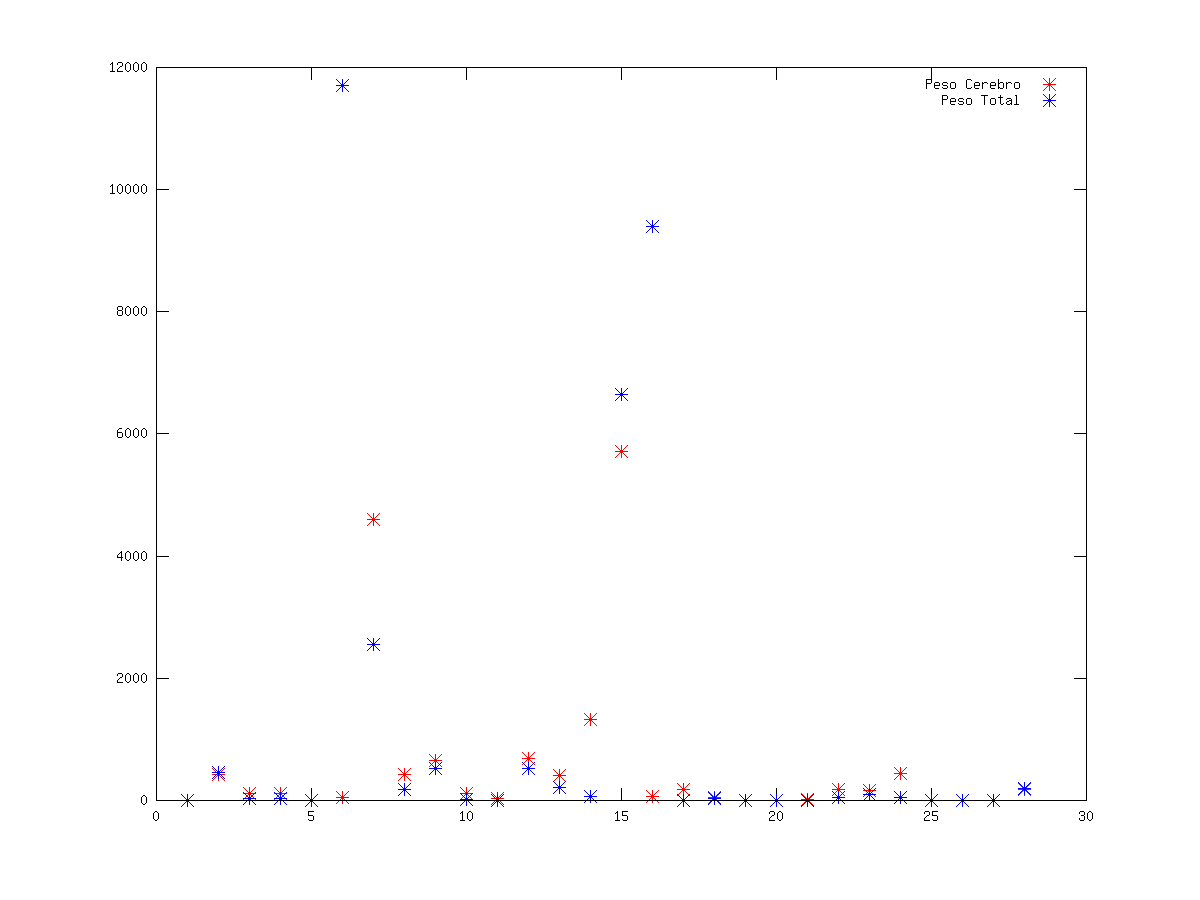
\includegraphics[scale=0.25]{TotalWeightVsBrainWeight}\caption{Peso del cerebro y peso total para cada medición en brains.txt{*}}
\end{figure}
\footnote{{*}El valor del peso del cerebro de la medición 25 no se ve en la
figura ya que se aleja demasiado del resto de los valores y el ajustar
los ejes solo para mostrar ese valor produce que todas las demas mediciónes
no puedan apreciarse correctamente.%
}


\begin{figure}[H]
\hspace{3cm}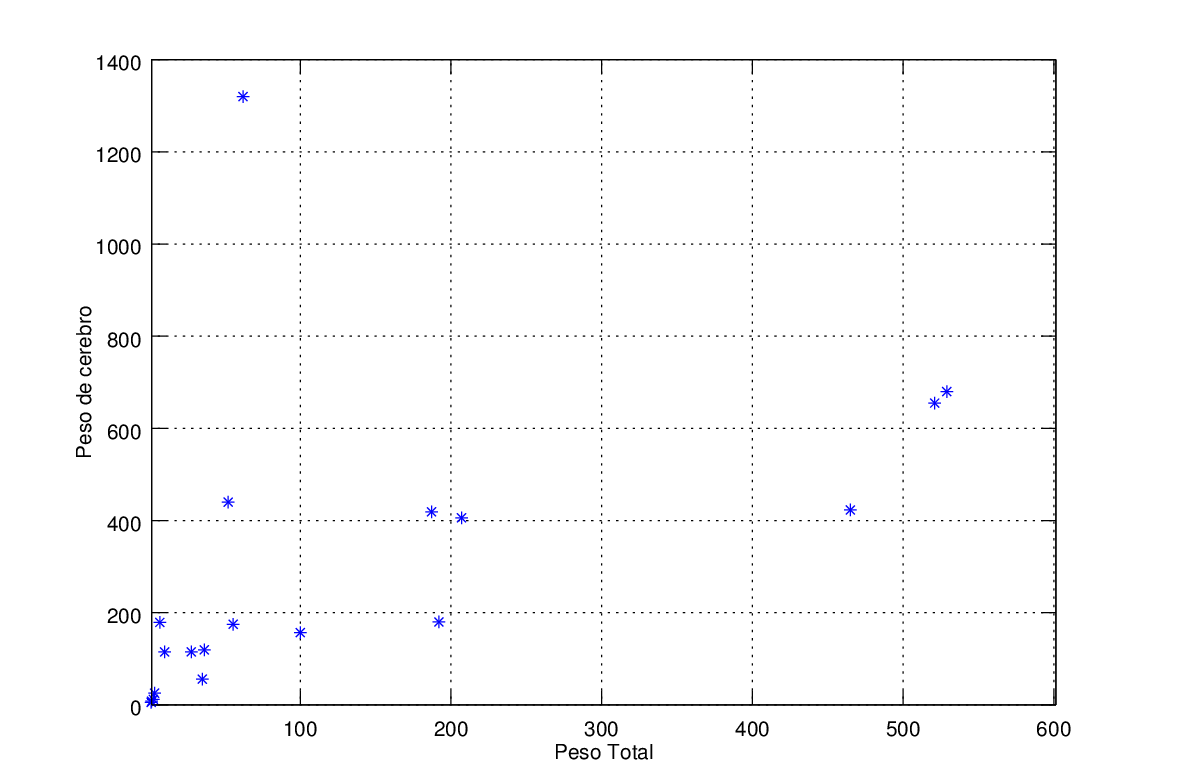
\includegraphics[scale=0.5]{TwVsBw}\caption{Peso total en Kg Vs peso del cerebro en G{*}{*}}
\end{figure}
\footnote{{*}{*}Se removieron los valores para los $4$ valores de $x$ mayores
a $2000$ ya que ocultaban la visualización de todos los demás valores%
}
\begin{enumerate}
\item En una observación a simple vista, se puede ver que las mediciónes
que se diferencian notablemente del resto son: $6,7,14,15,16$ y la
$25$.
\item En el segundo gráfico, puede verse que debido a la dispersión de los
datos, si aproximamos los valores por una recta, a simple vista se
ve que se va a estar cometiendo un error muy grande para la mayoría
de los datos. Por lo que no existe una relación lineal.
\end{enumerate}
\item En el gráfico a continuación puede verse que graficando el $log$
de ambas variables, los datos tienden a formar una línea mas definida. 

\begin{lyxcode}
\begin{figure}[H]
\centering{}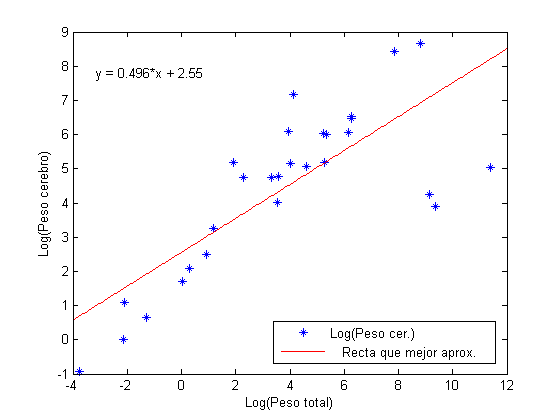
\includegraphics[scale=0.75]{logBrains}\caption{Logaritmo de ambas mediciónes y la línea que mejor los aproxima}
\end{figure}

\end{lyxcode}
\item La recta que mejor ajusta con los ejes $x$ e $y$ con la función
$log$ aplicados a ambos es: $y=a*x+b$. Con $a=0.496$ y $b=2.55$.
\\
Para obtener la recta que ajusta a los puntos $x$ e $y$ sin aplicar
las transformación, se debe aplicar la tranformación inversa al $log$,
es decir $pow(10,n)$. Quedando así la curva que aproxima a los puntos
como: $10^{y}=a*10^{x}+b$. Despejando por $y$, se obtiene $y=log(a*10^{x}+b)$. 

\begin{lyxcode}
\begin{center}
\begin{tabular}{|c|c|c|}
\hline 
Coeficientes de Regresion & $\sum res^{2}$ & $E_{cm}$\tabularnewline
\hline 
\hline 
0.496 - 2.55 & 60.99 & 2.34\tabularnewline
\hline 
\end{tabular}
\par\end{center}
\end{lyxcode}
\item En los gráficos del punto $b$, se puede observar que las mediciones
que estan muy fuera del común son no solo las$14,15$ y $25$ sinó
que también la $6$ y la $16$. Por lo que fueron removidos de la
tabla de valores. El gráfico obtenido luego de ajustados los valores
se muestra en la fiegura $5$ del Anexo.

\begin{lyxcode}
\begin{figure}[H]
\centering{}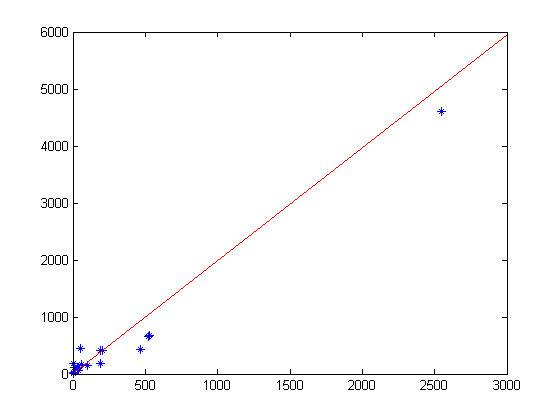
\includegraphics[scale=0.75]{outLayerRemovidos}\caption{Logaritmo de ambas mediciónes y la línea que mejor los aproxima}
\end{figure}

\end{lyxcode}
\end{enumerate}
\item Censo poblacional de Estados Unidos 1790 - 1990

\begin{enumerate}
\item 
\begin{figure}[H]
\begin{centering}
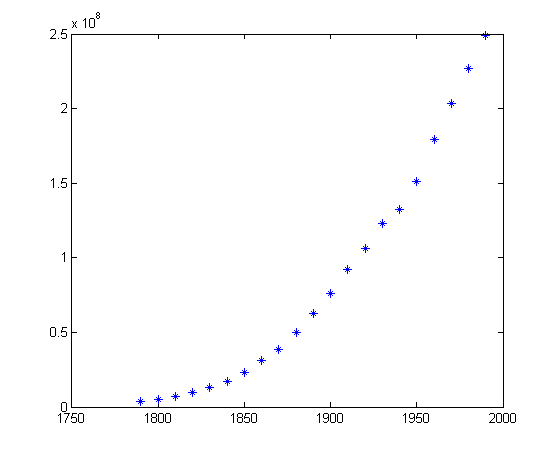
\includegraphics[scale=0.7]{population}\caption{Cantidad de habitantes medidas por el cendo por año}

\par\end{centering}

\end{figure}



De la figura puede verse que exite un patrón entre las mediciones,
pero no lineal.

\item $P_{2}(x)=p1*z^{2}+p2*z+p3$


$z=\frac{x-\mu}{\sigma}=\frac{x-1890}{62.05}$


$p1=2.5049e7$


$p2=7.5414e7$


$p3=6.1927e7$

\item $P_{3}(x)=p1*z^{3}+p2*z^{2}+p3*z+p4$


$p1=7.7279e5$


$p2=2.5049e7$


$p3=7.4093e7$


$p4=6.1927e7$

\item 
\begin{figure}[H]
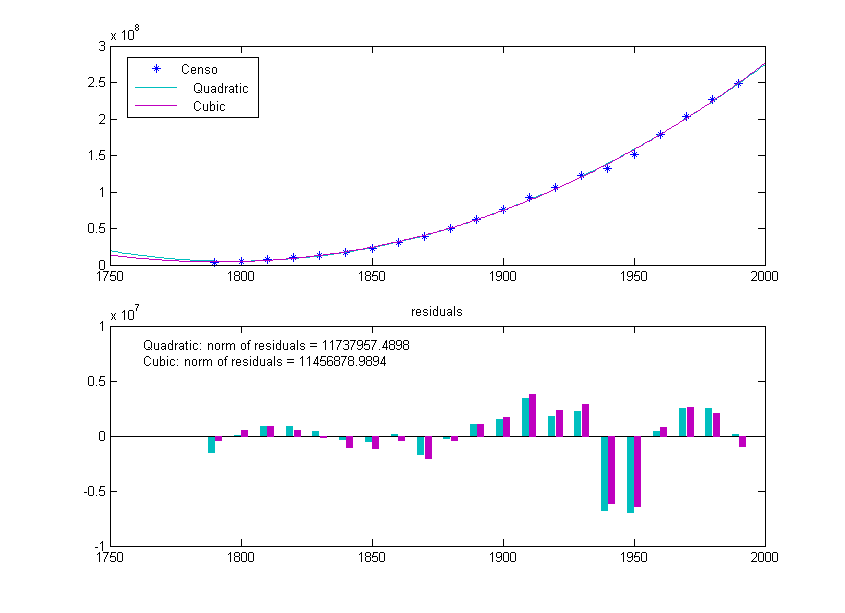
\includegraphics[scale=0.7]{populationBestFit}\caption{Cantidad de habitantes por cada año}
\end{figure}



A partir de los residuos generados por cada polinomio, puede verse
que el polinomio de grado $3$ es ligeramente menor, por lo que es
el que mejor representaría a esta muestra.

\item De acuerdo a cada polinomio, 


$P_{2}(2000)=2.74e8$


$P_{3}(2000)=2.76e8$


Sabiendo que el valor real para ese año fue $281421906$ ($2.8e8$).
Por haberle acertado con menor grado de error, el polinomio de grado
3 es el que mejor aproxima.

\end{enumerate}
\item Estimadores de maxima verosimilitud


\begin{center}
\begin{tabular}{|c|c|c|c|}
\hline 
Especie & Vector de medias {[}largo S., ancho S., largo P., ancho P.{]} & $\mu$ & $\sigma$\tabularnewline
\hline 
\hline 
Virginica & {[}6.5880, 2.9740, 5.5520, 2.0260{]} & 4.2850 & 3.4327\tabularnewline
\hline 
Versicolor & {[}5.9360, 2.7700, 4.2600, 1.3260{]} & 3.5730 & 3.5730\tabularnewline
\hline 
Setosa & {[}5.0060, 3.4280, 1.4620, 0.2460{]} & 2.5355 & 3.3235\tabularnewline
\hline 
\end{tabular}
\par\end{center}


\begin{center}
\begin{tabular}{|c|c|c|}
\hline 
Especie & Matriz de covarianza & $\sigma$\tabularnewline
\hline 
\hline 
Virgínica & %
\begin{tabular}{cccc}
0.4043 & 0.0938  & 0.3033  & 0.0491\tabularnewline
0.0938 & 0.1040 & 0.0714  & 0.0476 \tabularnewline
0.3033  & 0.0714  & 0.3046 &  0.0488\tabularnewline
0.0491  & 0.0476  & 0.0488  & 0.0754\tabularnewline
\end{tabular} & 0.8695\tabularnewline
\hline 
Versicolor & %
\begin{tabular}{cccc}
0.2664  & 0.0852  & 0.1829 &  0.0558\tabularnewline
0.0852 & 0.0985  & 0.0827 &  0.0412\tabularnewline
0.1829  & 0.0827  & 0.2208 &  0.0731\tabularnewline
0.0558  & 0.0412  & 0.0731  & 0.0391\tabularnewline
\end{tabular} & 0.6150\tabularnewline
\hline 
Setosa & %
\begin{tabular}{cccc}
0.1242 & 0.0992  & 0.0164  & 0.0103\tabularnewline
0.0992  & 0.1437  & 0.0117 &  0.0093\tabularnewline
0.0164  & 0.0117  & 0.0302  & 0.0061\tabularnewline
0.0103 & 0.0093  & 0.0061  & 0.0111\tabularnewline
\end{tabular} & 0.3064\tabularnewline
\hline 
\end{tabular}
\par\end{center}

\item Matriz obtenida:

\begin{enumerate}
\item %
\begin{tabular}{|c|c|c|c|}
\hline 
1 & 0.2286 & -0.8241  & -0.2454\tabularnewline
\hline 
0.2286 & 1  & -0.1392 &  -0.9730\tabularnewline
\hline 
-0.8241 & -0.1392 & 1  & 0.0295\tabularnewline
\hline 
-0.2454  & -0.9730 & 0.0295  & 1\tabularnewline
\hline 
\end{tabular}


Cada $x_{ij}$ representa la correlación de la cantidad de calor por
ingrediente $i$ por gramo de cemento con relacion al elemento $j$.
Cuanto mas cercano em módulo a 1 es, mas se correlacionan.

\item selección hacia adelante


\begin{center}
\begin{tabular}{|c|c|c|}
\hline 
 & $R^{2}$ & $F$\tabularnewline
\hline 
\hline 
$x_{1}$ & 0.5339  & 12.6025\tabularnewline
\hline 
$x_{2}$ & 0.6663  & 21.9606\tabularnewline
\hline 
$x_{3}$ & 0.2859  & 4.4034\tabularnewline
\hline 
$x_{4}$ & \textcolor{blue}{0.6745 } & \textcolor{blue}{22.7985}\tabularnewline
\hline 
\end{tabular}$\Longrightarrow$%
\begin{tabular}{|c|c|c|}
\hline 
 & $R^{2}$ & $F$\tabularnewline
\hline 
\hline 
$x_{4}x_{1}$ & \textcolor{blue}{0.9725} & \textcolor{blue}{{} 176.6270}\tabularnewline
\hline 
$x_{4}x_{2}$ & 0.6801  & 10.6280\tabularnewline
\hline 
$x_{4}x_{3}$ & 0.9353  & 72.2674\tabularnewline
\hline 
\end{tabular}$\Longrightarrow$%
\begin{tabular}{|c|c|c|}
\hline 
 & $R^{2}$ & $F$\tabularnewline
\hline 
\hline 
$x_{1}x_{4}x_{2}$ & \textcolor{blue}{0.9823 } & \textcolor{blue}{166.8317}\tabularnewline
\hline 
$x_{1}x_{4}x_{3}$ & 0.9813 & 157.2658\tabularnewline
\hline 
\end{tabular}
\par\end{center}

\end{enumerate}
\item Proporción de la varianza = $\frac{\lambda_{1}+...+\lambda_{k}}{\lambda_{1}+...+\lambda_{p}}$
para cada una de las variables:


1 variable: 0.8660


2 variables:\textcolor{blue}{{} 0.9789} 


3 variables:\textcolor{blue}{{} }0.9996


4 variables:\textcolor{blue}{{} }1


Del análisis de los autovalores de la matriz de covarianza se puede
ver que solamente con $2$ componentes, es posible representar mas
del $90\%$ de la varianza.

\end{enumerate}
\begin{lyxcode}
\newpage{}
\end{lyxcode}

\section{Anexo}
\begin{enumerate}
\item Lirios Fisher

\begin{enumerate}
\item Código

\begin{lyxcode}
\%range~toma~los~valores~0:50;~51:100~y~101:150

data=meas(range,:);

n=size(data,1);

uHat=mean(data);

sHat=(n-1){*}std(range)/n;
\end{lyxcode}
\item Código

\begin{lyxcode}
ecm=std(data).\textasciicircum{}2;

ecm=ecm/n;
\end{lyxcode}
\item Código

\begin{lyxcode}
mu=mean(data);

sigma=std(data);

p=0.05/2;

zAlpha=tinv(p,n-1)~\%~T~student

aux=zAlpha.{*}sigma/sqrt(n);

interval={[}mu-aux,mu+aux{]};
\end{lyxcode}
\end{enumerate}
\item -
\item Carpinteros escapularios

\begin{lyxcode}
birds={[}~

~~~...meditions~here...

{]};

alpha=0.05\};

{[}h,p,ci,stats{]}=ttest(birds(:,2),birds(:,3),alpha);
\end{lyxcode}
\item Masa croporal vs Masa cerebral

\begin{enumerate}
\item Código

\begin{lyxcode}
load~brains.txt;

x~=~1:28;

y~=~brains(:,1);

z~=~brains(:,2);

clf;

hold~on;

plot(x,~y,~'{*}b;Peso~Promedio~en~Kg;')

plot(x,~z,~'{*}r;Peso~Cerebro~Promedio~en~G;')

print('-dpng',~'./TotalWeightVsBrainWeight.png')
\end{lyxcode}
\item Código

\begin{lyxcode}
load~brains.txt~

regstats(brains(:,1),~brains(:,2),'línear')
\end{lyxcode}
\end{enumerate}
\item Censo

\begin{enumerate}
\item .

\begin{lyxcode}
load~population.txt;~

x~=~population(:,~1);~

y~=~population(:,~2);~

plot(x,y,~'{*}')
\end{lyxcode}
\item .

\begin{lyxcode}
load~population.txt;

c2=polyfit(cdate,pop,2)

poli2=polyval(c2,cdate);
\end{lyxcode}
\end{enumerate}
\item Lirios Fisher

\begin{lyxcode}
meanVector=mean(data)

n=size(meanVector,2);

mu=mean(meanVector)

sigma=~sum((meanVector-ones(1,n){*}mu).\textasciicircum{}2)/n~\\
\%~segunda~parte

cm=cov(data)

sigma=cm(1,1)+cm(2,2)+cm(3,3)+cm(4,4){*}(n-1)/n
\end{lyxcode}
\item Evolución de las calorías por gramo de cemento

\begin{lyxcode}
{[}r{]}~=~corrcoef(ingredients)\end{lyxcode}
\end{enumerate}

\end{document}
